% Options for packages loaded elsewhere
\PassOptionsToPackage{unicode}{hyperref}
\PassOptionsToPackage{hyphens}{url}
\PassOptionsToPackage{dvipsnames,svgnames,x11names}{xcolor}
%
\documentclass[
  letterpaper,
  DIV=11,
  numbers=noendperiod]{scrartcl}

\usepackage{amsmath,amssymb}
\usepackage{iftex}
\ifPDFTeX
  \usepackage[T1]{fontenc}
  \usepackage[utf8]{inputenc}
  \usepackage{textcomp} % provide euro and other symbols
\else % if luatex or xetex
  \usepackage{unicode-math}
  \defaultfontfeatures{Scale=MatchLowercase}
  \defaultfontfeatures[\rmfamily]{Ligatures=TeX,Scale=1}
\fi
\usepackage{lmodern}
\ifPDFTeX\else  
    % xetex/luatex font selection
\fi
% Use upquote if available, for straight quotes in verbatim environments
\IfFileExists{upquote.sty}{\usepackage{upquote}}{}
\IfFileExists{microtype.sty}{% use microtype if available
  \usepackage[]{microtype}
  \UseMicrotypeSet[protrusion]{basicmath} % disable protrusion for tt fonts
}{}
\makeatletter
\@ifundefined{KOMAClassName}{% if non-KOMA class
  \IfFileExists{parskip.sty}{%
    \usepackage{parskip}
  }{% else
    \setlength{\parindent}{0pt}
    \setlength{\parskip}{6pt plus 2pt minus 1pt}}
}{% if KOMA class
  \KOMAoptions{parskip=half}}
\makeatother
\usepackage{xcolor}
\setlength{\emergencystretch}{3em} % prevent overfull lines
\setcounter{secnumdepth}{-\maxdimen} % remove section numbering
% Make \paragraph and \subparagraph free-standing
\ifx\paragraph\undefined\else
  \let\oldparagraph\paragraph
  \renewcommand{\paragraph}[1]{\oldparagraph{#1}\mbox{}}
\fi
\ifx\subparagraph\undefined\else
  \let\oldsubparagraph\subparagraph
  \renewcommand{\subparagraph}[1]{\oldsubparagraph{#1}\mbox{}}
\fi

\usepackage{color}
\usepackage{fancyvrb}
\newcommand{\VerbBar}{|}
\newcommand{\VERB}{\Verb[commandchars=\\\{\}]}
\DefineVerbatimEnvironment{Highlighting}{Verbatim}{commandchars=\\\{\}}
% Add ',fontsize=\small' for more characters per line
\usepackage{framed}
\definecolor{shadecolor}{RGB}{241,243,245}
\newenvironment{Shaded}{\begin{snugshade}}{\end{snugshade}}
\newcommand{\AlertTok}[1]{\textcolor[rgb]{0.68,0.00,0.00}{#1}}
\newcommand{\AnnotationTok}[1]{\textcolor[rgb]{0.37,0.37,0.37}{#1}}
\newcommand{\AttributeTok}[1]{\textcolor[rgb]{0.40,0.45,0.13}{#1}}
\newcommand{\BaseNTok}[1]{\textcolor[rgb]{0.68,0.00,0.00}{#1}}
\newcommand{\BuiltInTok}[1]{\textcolor[rgb]{0.00,0.23,0.31}{#1}}
\newcommand{\CharTok}[1]{\textcolor[rgb]{0.13,0.47,0.30}{#1}}
\newcommand{\CommentTok}[1]{\textcolor[rgb]{0.37,0.37,0.37}{#1}}
\newcommand{\CommentVarTok}[1]{\textcolor[rgb]{0.37,0.37,0.37}{\textit{#1}}}
\newcommand{\ConstantTok}[1]{\textcolor[rgb]{0.56,0.35,0.01}{#1}}
\newcommand{\ControlFlowTok}[1]{\textcolor[rgb]{0.00,0.23,0.31}{#1}}
\newcommand{\DataTypeTok}[1]{\textcolor[rgb]{0.68,0.00,0.00}{#1}}
\newcommand{\DecValTok}[1]{\textcolor[rgb]{0.68,0.00,0.00}{#1}}
\newcommand{\DocumentationTok}[1]{\textcolor[rgb]{0.37,0.37,0.37}{\textit{#1}}}
\newcommand{\ErrorTok}[1]{\textcolor[rgb]{0.68,0.00,0.00}{#1}}
\newcommand{\ExtensionTok}[1]{\textcolor[rgb]{0.00,0.23,0.31}{#1}}
\newcommand{\FloatTok}[1]{\textcolor[rgb]{0.68,0.00,0.00}{#1}}
\newcommand{\FunctionTok}[1]{\textcolor[rgb]{0.28,0.35,0.67}{#1}}
\newcommand{\ImportTok}[1]{\textcolor[rgb]{0.00,0.46,0.62}{#1}}
\newcommand{\InformationTok}[1]{\textcolor[rgb]{0.37,0.37,0.37}{#1}}
\newcommand{\KeywordTok}[1]{\textcolor[rgb]{0.00,0.23,0.31}{#1}}
\newcommand{\NormalTok}[1]{\textcolor[rgb]{0.00,0.23,0.31}{#1}}
\newcommand{\OperatorTok}[1]{\textcolor[rgb]{0.37,0.37,0.37}{#1}}
\newcommand{\OtherTok}[1]{\textcolor[rgb]{0.00,0.23,0.31}{#1}}
\newcommand{\PreprocessorTok}[1]{\textcolor[rgb]{0.68,0.00,0.00}{#1}}
\newcommand{\RegionMarkerTok}[1]{\textcolor[rgb]{0.00,0.23,0.31}{#1}}
\newcommand{\SpecialCharTok}[1]{\textcolor[rgb]{0.37,0.37,0.37}{#1}}
\newcommand{\SpecialStringTok}[1]{\textcolor[rgb]{0.13,0.47,0.30}{#1}}
\newcommand{\StringTok}[1]{\textcolor[rgb]{0.13,0.47,0.30}{#1}}
\newcommand{\VariableTok}[1]{\textcolor[rgb]{0.07,0.07,0.07}{#1}}
\newcommand{\VerbatimStringTok}[1]{\textcolor[rgb]{0.13,0.47,0.30}{#1}}
\newcommand{\WarningTok}[1]{\textcolor[rgb]{0.37,0.37,0.37}{\textit{#1}}}

\providecommand{\tightlist}{%
  \setlength{\itemsep}{0pt}\setlength{\parskip}{0pt}}\usepackage{longtable,booktabs,array}
\usepackage{calc} % for calculating minipage widths
% Correct order of tables after \paragraph or \subparagraph
\usepackage{etoolbox}
\makeatletter
\patchcmd\longtable{\par}{\if@noskipsec\mbox{}\fi\par}{}{}
\makeatother
% Allow footnotes in longtable head/foot
\IfFileExists{footnotehyper.sty}{\usepackage{footnotehyper}}{\usepackage{footnote}}
\makesavenoteenv{longtable}
\usepackage{graphicx}
\makeatletter
\def\maxwidth{\ifdim\Gin@nat@width>\linewidth\linewidth\else\Gin@nat@width\fi}
\def\maxheight{\ifdim\Gin@nat@height>\textheight\textheight\else\Gin@nat@height\fi}
\makeatother
% Scale images if necessary, so that they will not overflow the page
% margins by default, and it is still possible to overwrite the defaults
% using explicit options in \includegraphics[width, height, ...]{}
\setkeys{Gin}{width=\maxwidth,height=\maxheight,keepaspectratio}
% Set default figure placement to htbp
\makeatletter
\def\fps@figure{htbp}
\makeatother

\KOMAoption{captions}{tableheading}
\makeatletter
\makeatother
\makeatletter
\makeatother
\makeatletter
\@ifpackageloaded{caption}{}{\usepackage{caption}}
\AtBeginDocument{%
\ifdefined\contentsname
  \renewcommand*\contentsname{Table of contents}
\else
  \newcommand\contentsname{Table of contents}
\fi
\ifdefined\listfigurename
  \renewcommand*\listfigurename{List of Figures}
\else
  \newcommand\listfigurename{List of Figures}
\fi
\ifdefined\listtablename
  \renewcommand*\listtablename{List of Tables}
\else
  \newcommand\listtablename{List of Tables}
\fi
\ifdefined\figurename
  \renewcommand*\figurename{Figure}
\else
  \newcommand\figurename{Figure}
\fi
\ifdefined\tablename
  \renewcommand*\tablename{Table}
\else
  \newcommand\tablename{Table}
\fi
}
\@ifpackageloaded{float}{}{\usepackage{float}}
\floatstyle{ruled}
\@ifundefined{c@chapter}{\newfloat{codelisting}{h}{lop}}{\newfloat{codelisting}{h}{lop}[chapter]}
\floatname{codelisting}{Listing}
\newcommand*\listoflistings{\listof{codelisting}{List of Listings}}
\makeatother
\makeatletter
\@ifpackageloaded{caption}{}{\usepackage{caption}}
\@ifpackageloaded{subcaption}{}{\usepackage{subcaption}}
\makeatother
\makeatletter
\@ifpackageloaded{tcolorbox}{}{\usepackage[skins,breakable]{tcolorbox}}
\makeatother
\makeatletter
\@ifundefined{shadecolor}{\definecolor{shadecolor}{rgb}{.97, .97, .97}}
\makeatother
\makeatletter
\makeatother
\makeatletter
\makeatother
\ifLuaTeX
  \usepackage{selnolig}  % disable illegal ligatures
\fi
\IfFileExists{bookmark.sty}{\usepackage{bookmark}}{\usepackage{hyperref}}
\IfFileExists{xurl.sty}{\usepackage{xurl}}{} % add URL line breaks if available
\urlstyle{same} % disable monospaced font for URLs
\hypersetup{
  pdftitle={Yellow Tulip Post Event Survey Analysis - 2022/2023},
  pdfauthor={Robert Szarek},
  colorlinks=true,
  linkcolor={blue},
  filecolor={Maroon},
  citecolor={Blue},
  urlcolor={Blue},
  pdfcreator={LaTeX via pandoc}}

\title{Yellow Tulip Post Event Survey Analysis - 2022/2023}
\author{Robert Szarek}
\date{}

\begin{document}
\maketitle
\ifdefined\Shaded\renewenvironment{Shaded}{\begin{tcolorbox}[interior hidden, breakable, frame hidden, borderline west={3pt}{0pt}{shadecolor}, sharp corners, boxrule=0pt, enhanced]}{\end{tcolorbox}}\fi

\hypertarget{introduction}{%
\section{Introduction}\label{introduction}}

This report is dynamic; it auto-updates itself whenever you have a
refreshed dataset with survey responses. The first stage of running
analyses for YTP includes getting a sense for the different datasets.
The second stage will be to auto-update the data and track it in real
time to provide refreshed analyses. First however, we need to agree upon
what exactly we'd like to report out on, and part of that is to demo the
visualizations we can render in R.

\hypertarget{document-setup}{%
\section{Document Setup}\label{document-setup}}

Our analysis relies on several external packages, these are listed in
the code snippet below. For your information, code snippets help the
reader better understand how a particular visualization or data cleaning
step was conducted; it makes the research reproducible.

\begin{Shaded}
\begin{Highlighting}[]
\FunctionTok{library}\NormalTok{(tinytex)}
\FunctionTok{library}\NormalTok{(readr)}
\FunctionTok{library}\NormalTok{(dplyr)}
\FunctionTok{library}\NormalTok{(tidyr)}
\FunctionTok{library}\NormalTok{(ggplot2)}
\FunctionTok{library}\NormalTok{(tidytext)}
\FunctionTok{library}\NormalTok{(stringr)}
\FunctionTok{library}\NormalTok{(wordcloud)}
\FunctionTok{library}\NormalTok{(SnowballC)}
\FunctionTok{library}\NormalTok{(corrplot)}
\end{Highlighting}
\end{Shaded}

\hypertarget{data-ingestion}{%
\section{Data Ingestion}\label{data-ingestion}}

We read in our data with the code snippet below. Moving forward, we'd
like to directly connect to \emph{Google Sheets} using the package
\texttt{googlesheets4} to establish a straight connection and refresh
this analysis whenever we'd like.

\begin{Shaded}
\begin{Highlighting}[]
\NormalTok{df\_pe\_survey }\OtherTok{\textless{}{-}}\NormalTok{ readr}\SpecialCharTok{::}\FunctionTok{read\_csv}\NormalTok{(}\AttributeTok{file =} \StringTok{\textquotesingle{}/Users/rszarek/Library/CloudStorage/OneDrive{-}Unum/Projects/ytp\_cdp\_analysis/data/YTP Post Event Survey (Responses) {-} Form Responses 1.csv\textquotesingle{}}\NormalTok{)}
\end{Highlighting}
\end{Shaded}

\hypertarget{data-engineering}{%
\subsection{Data Engineering}\label{data-engineering}}

We first need to clean up some of the columns, because the variable
names are either too lengthy, or the type of the variable is improper,
we do that with the code below:

\begin{Shaded}
\begin{Highlighting}[]
\NormalTok{df\_pe\_survey\_clean }\OtherTok{\textless{}{-}}
\NormalTok{  df\_pe\_survey }\SpecialCharTok{|\textgreater{}} 
  \FunctionTok{rename}\NormalTok{(}
    \AttributeTok{Date =}\NormalTok{ Timestamp,}
    \AttributeTok{Event\_Date =} \StringTok{"2. Date of Event"}\NormalTok{,}
    \AttributeTok{Race =} \StringTok{"12. How do you identify racially? Please check all that apply."}\NormalTok{,}
    \AttributeTok{Age =} \StringTok{"11. What is your age?"}\NormalTok{,}
    \AttributeTok{Zipcode =} \StringTok{"10. What is your ZIP code?"}\NormalTok{,}
    \AttributeTok{Event =} \StringTok{"1. Which YTP event are you completing this survey for? Please check all that apply."}\NormalTok{,}
    \AttributeTok{Join\_Network =} \StringTok{"YTP has (3) networks–Youth, Community + Educator. Are you interested in joi"}\NormalTok{,}
    \AttributeTok{Hear\_ytp =} \StringTok{"9. How did you hear about The Yellow Tulip Project?"}\NormalTok{,}
    \AttributeTok{Connected =} \StringTok{"3. This event helps me feel more connected to my community."}\NormalTok{,}
    \AttributeTok{Reduce\_Stigma =} \StringTok{"5. This event helps reduce the stigma associated with mental illness."}\NormalTok{,}
    \AttributeTok{More\_Hopeful =} \StringTok{"4. This event helps me feel more hopeful."}\NormalTok{,}
    \AttributeTok{Text\_Improve =} \StringTok{"8. We want our programming to be as meaningful and engaging as it can be for everyone. Please let us know how we could have improved your experience."}\NormalTok{,}
    \AttributeTok{Educator =} \StringTok{"14. Are you an educator (i.e. school nurse, social worker, teacher, professor etc.)?"}\NormalTok{,}
    \AttributeTok{Email =} \StringTok{"Email Address"}\NormalTok{,}
    \AttributeTok{Gender =} \StringTok{"13. How do you define your gender identity? Please check all that apply."}\NormalTok{,}
    \AttributeTok{Future\_Attend =} \StringTok{"6. How likely would you be to attend a future YTP event?"}\NormalTok{,}
    \AttributeTok{Recommend =} \StringTok{"7. How likely would you be to recommend the event to a friend?"}
\NormalTok{  ) }\SpecialCharTok{|\textgreater{}} 
  \FunctionTok{mutate}\NormalTok{(}\AttributeTok{Age =} \FunctionTok{as.double}\NormalTok{(Age)) }\SpecialCharTok{|\textgreater{}} 
  \FunctionTok{mutate}\NormalTok{(}\AttributeTok{Age\_Bin =} \FunctionTok{ifelse}\NormalTok{(Age }\SpecialCharTok{\textless{}} \DecValTok{40}\NormalTok{, }\StringTok{\textquotesingle{}\textless{}40\textquotesingle{}}\NormalTok{, }\StringTok{\textquotesingle{}\textgreater{}40\textquotesingle{}}\NormalTok{)) }\SpecialCharTok{|\textgreater{}} 
  \FunctionTok{mutate}\NormalTok{(}\AttributeTok{Zipcode =} \FunctionTok{as.character}\NormalTok{(stringr}\SpecialCharTok{::}\FunctionTok{str\_extract}\NormalTok{(Zipcode, }\StringTok{"}\SpecialCharTok{\textbackslash{}\textbackslash{}}\StringTok{d+.}\SpecialCharTok{\textbackslash{}\textbackslash{}}\StringTok{d+"}\NormalTok{)))}
\end{Highlighting}
\end{Shaded}

Next, we need to factorise the Likert scale options. This factorisation
primarily focuses us to transform text into numeric values, so that we
are then able to run descriptive statistics on the resultant data and
run comparisons across the different demographic partitions:

\begin{Shaded}
\begin{Highlighting}[]
\NormalTok{scale\_factorise }\OtherTok{\textless{}{-}} \ControlFlowTok{function}\NormalTok{(x) \{}
  \FunctionTok{case\_when}\NormalTok{(x }\SpecialCharTok{==} \StringTok{\textquotesingle{}Strongly Agree\textquotesingle{}} \SpecialCharTok{|}\NormalTok{ x }\SpecialCharTok{==} \StringTok{\textquotesingle{}Very likely\textquotesingle{}} \SpecialCharTok{\textasciitilde{}} \DecValTok{5}\NormalTok{,}
\NormalTok{            x }\SpecialCharTok{==} \StringTok{\textquotesingle{}Agree\textquotesingle{}} \SpecialCharTok{|}\NormalTok{ x }\SpecialCharTok{==} \StringTok{\textquotesingle{}Likely\textquotesingle{}} \SpecialCharTok{\textasciitilde{}} \DecValTok{4}\NormalTok{,}
\NormalTok{            x }\SpecialCharTok{==} \StringTok{\textquotesingle{}Neutral\textquotesingle{}} \SpecialCharTok{\textasciitilde{}} \DecValTok{3}\NormalTok{,}
\NormalTok{            x }\SpecialCharTok{==} \StringTok{\textquotesingle{}Somewhat disagree\textquotesingle{}} \SpecialCharTok{|}\NormalTok{ x }\SpecialCharTok{==} \StringTok{\textquotesingle{}Unlikely\textquotesingle{}} \SpecialCharTok{\textasciitilde{}} \DecValTok{2}\NormalTok{,}
\NormalTok{            x }\SpecialCharTok{==} \StringTok{\textquotesingle{}Strongly Disagree\textquotesingle{}} \SpecialCharTok{|}\NormalTok{ x }\SpecialCharTok{==} \StringTok{\textquotesingle{}Not likely at all\textquotesingle{}} \SpecialCharTok{\textasciitilde{}} \DecValTok{1}\NormalTok{)}
\NormalTok{\}}

\NormalTok{df\_pe\_survey\_clean }\OtherTok{\textless{}{-}}
\NormalTok{df\_pe\_survey\_clean }\SpecialCharTok{|\textgreater{}} 
  \FunctionTok{mutate}\NormalTok{(}\AttributeTok{Connected =} \FunctionTok{scale\_factorise}\NormalTok{(Connected),}
         \AttributeTok{Reduce\_Stigma =} \FunctionTok{scale\_factorise}\NormalTok{(Reduce\_Stigma),}
         \AttributeTok{More\_Hopeful =} \FunctionTok{scale\_factorise}\NormalTok{(More\_Hopeful),}
         \AttributeTok{Future\_Attend =} \FunctionTok{scale\_factorise}\NormalTok{(Future\_Attend),}
         \AttributeTok{Recommend =} \FunctionTok{scale\_factorise}\NormalTok{(Recommend))}
\end{Highlighting}
\end{Shaded}

\hypertarget{descriptive-statistics}{%
\subsection{Descriptive Statistics}\label{descriptive-statistics}}

Descriptive statistics primarily deal with counts. Here we count the
number of observations in our particular demographic responses to better
understand the composition of our sample size.

\hypertarget{zipcode}{%
\subsubsection{Zipcode}\label{zipcode}}

\begin{Shaded}
\begin{Highlighting}[]
\NormalTok{df\_pe\_survey\_clean }\SpecialCharTok{|\textgreater{}} 
  \FunctionTok{count}\NormalTok{(Zipcode, }\AttributeTok{sort =} \ConstantTok{TRUE}\NormalTok{)}
\end{Highlighting}
\end{Shaded}

\begin{verbatim}
# A tibble: 21 x 2
   Zipcode     n
   <chr>   <int>
 1 02360       8
 2 06830       8
 3 <NA>        5
 4 01588       3
 5 04090       2
 6 15206       2
 7 01534       1
 8 01584       1
 9 01610       1
10 02332       1
# i 11 more rows
\end{verbatim}

\begin{Shaded}
\begin{Highlighting}[]
\NormalTok{df\_pe\_survey\_clean }\OtherTok{\textless{}{-}}
\NormalTok{  df\_pe\_survey\_clean }\SpecialCharTok{|\textgreater{}} 
  \FunctionTok{mutate}\NormalTok{(}\AttributeTok{City =} \FunctionTok{case\_when}\NormalTok{(Zipcode }\SpecialCharTok{==} \StringTok{\textquotesingle{}02360\textquotesingle{}} \SpecialCharTok{\textasciitilde{}} \StringTok{\textquotesingle{}Plymouth, MA\textquotesingle{}}\NormalTok{,}
\NormalTok{                          Zipcode }\SpecialCharTok{==} \StringTok{\textquotesingle{}06830\textquotesingle{}} \SpecialCharTok{\textasciitilde{}} \StringTok{\textquotesingle{}Greenwich, CT\textquotesingle{}}\NormalTok{,}
                          \ConstantTok{TRUE} \SpecialCharTok{\textasciitilde{}} \ConstantTok{NA}\NormalTok{))}
\end{Highlighting}
\end{Shaded}

A majority of respondents came from two zipcodes: 02360 and 06830. This
is Plymouth, MA and Greenwich, CT. The remainder of the zipcodes are
from surrounding areas.

\hypertarget{age}{%
\subsubsection{Age}\label{age}}

We take a look at the distribution of age in our survey:

\begin{Shaded}
\begin{Highlighting}[]
\FunctionTok{ggplot}\NormalTok{(df\_pe\_survey\_clean, }\FunctionTok{aes}\NormalTok{(}\AttributeTok{x=}\NormalTok{Age))}\SpecialCharTok{+}
  \FunctionTok{geom\_histogram}\NormalTok{(}\AttributeTok{color=}\StringTok{"darkblue"}\NormalTok{, }\AttributeTok{fill=}\StringTok{"lightblue"}\NormalTok{, }\AttributeTok{binwidth =}  \DecValTok{3}\NormalTok{)}
\end{Highlighting}
\end{Shaded}

\begin{figure}[H]

{\centering 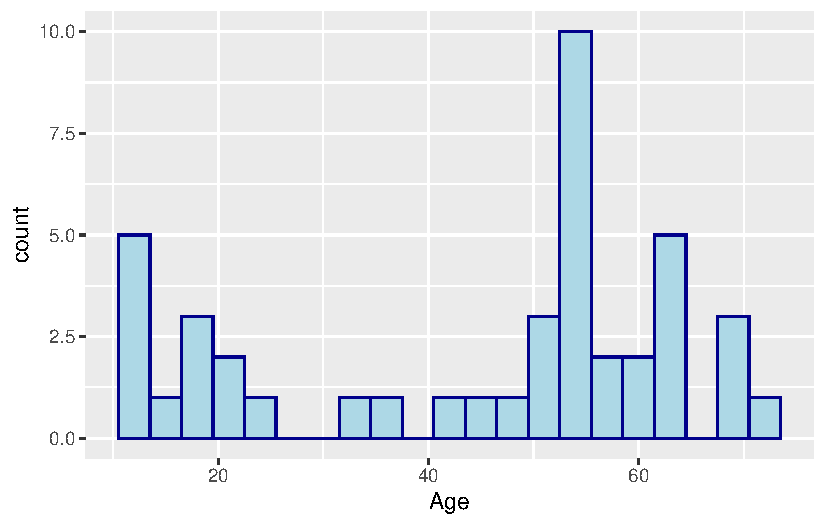
\includegraphics{ytp_post_event_survey_files/figure-pdf/unnamed-chunk-6-1.pdf}

}

\end{figure}

This is a very interesting graphic. We can see that the distribution of
our sample is split between around \textless{} 40 years of age and
\textgreater{} 40 years of age. Therefore, I think it makes sense that
the conclusion of this survey regarding the age of the participants is
that we are targeting both groups of people, young and elderly. For the
purposes of binning the age variable, we should have 40 be the cut-off
point.

\hypertarget{heard-about-ytp}{%
\subsubsection{Heard about YTP}\label{heard-about-ytp}}

The three primary ``ways'' that people hear about Yellow Tulip events is
through a friend, their school, or work. This is evidenced in the
counts:

\begin{Shaded}
\begin{Highlighting}[]
\NormalTok{df\_pe\_survey\_clean }\SpecialCharTok{|\textgreater{}} 
  \FunctionTok{count}\NormalTok{(Hear\_ytp, }\AttributeTok{sort =} \ConstantTok{TRUE}\NormalTok{) }\SpecialCharTok{|\textgreater{}} 
  \FunctionTok{filter}\NormalTok{(n }\SpecialCharTok{\textgreater{}} \DecValTok{5}\NormalTok{)}
\end{Highlighting}
\end{Shaded}

\begin{verbatim}
# A tibble: 3 x 2
  Hear_ytp     n
  <chr>    <int>
1 Friend      10
2 School      10
3 Work         9
\end{verbatim}

The only other metric I would track for how people heard about YTP would
be social media. Though in the current iteration, this does not seem to
be a very high volume of people coming in through social media. This may
change in the future, however.

\hypertarget{gender}{%
\subsubsection{Gender}\label{gender}}

\begin{Shaded}
\begin{Highlighting}[]
\NormalTok{df\_pe\_survey\_clean }\SpecialCharTok{|\textgreater{}} 
  \FunctionTok{count}\NormalTok{(Gender)}
\end{Highlighting}
\end{Shaded}

\begin{verbatim}
# A tibble: 3 x 2
  Gender     n
  <chr>  <int>
1 Female    14
2 Male       4
3 <NA>      25
\end{verbatim}

We had a glitch in the data that has produced a lot of NA values. I
believe moving forward this has been corrected. According to the current
data, a majority of the survey responses were from females. making up
about 75\% of the total sample.

\hypertarget{race}{%
\subsubsection{Race}\label{race}}

We take a look at our survey responses by Race:

\begin{Shaded}
\begin{Highlighting}[]
\NormalTok{df\_pe\_survey\_clean }\SpecialCharTok{|\textgreater{}} 
  \FunctionTok{count}\NormalTok{(Race, }\AttributeTok{sort =} \ConstantTok{TRUE}\NormalTok{)}
\end{Highlighting}
\end{Shaded}

\begin{verbatim}
# A tibble: 20 x 2
   Race                                       n
   <chr>                                  <int>
 1 White                                     15
 2 10/6/2022                                  4
 3 4/23/2022                                  4
 4 10/8/2022                                  3
 5 5/21/2022                                  2
 6 10/1/2022                                  1
 7 10/10/2022                                 1
 8 10/12/2022                                 1
 9 10/19/2022                                 1
10 10/8/0022                                  1
11 4/11/2022                                  1
12 4/22/2022                                  1
13 4/25/2022                                  1
14 4/28/2022                                  1
15 5/1/2022                                   1
16 5/20/2022                                  1
17 5/21/2023                                  1
18 Black or African American                  1
19 Latinx/Latine/Hispanic, White              1
20 White, Native American/American Indian     1
\end{verbatim}

Unfortunately, a glitch in the data has caused us to mix dates with race
information. We need to filter out the dates:

\begin{Shaded}
\begin{Highlighting}[]
\NormalTok{df\_pe\_survey\_clean }\SpecialCharTok{|\textgreater{}} 
  \FunctionTok{filter}\NormalTok{(}\SpecialCharTok{!}\NormalTok{stringr}\SpecialCharTok{::}\FunctionTok{str\_detect}\NormalTok{(Race, }\StringTok{\textquotesingle{}2021|2022|2023|0022\textquotesingle{}}\NormalTok{)) }\SpecialCharTok{|\textgreater{}} 
  \FunctionTok{count}\NormalTok{(Race, }\AttributeTok{sort=}\ConstantTok{TRUE}\NormalTok{)}
\end{Highlighting}
\end{Shaded}

\begin{verbatim}
# A tibble: 4 x 2
  Race                                       n
  <chr>                                  <int>
1 White                                     15
2 Black or African American                  1
3 Latinx/Latine/Hispanic, White              1
4 White, Native American/American Indian     1
\end{verbatim}

After filtering, our primary composition of attendees is White. With a
single participant for Black, Latinx, and Native American.

\hypertarget{joining-network}{%
\subsubsection{Joining Network}\label{joining-network}}

\begin{Shaded}
\begin{Highlighting}[]
\NormalTok{df\_pe\_survey\_clean }\SpecialCharTok{|\textgreater{}} 
  \FunctionTok{count}\NormalTok{(Join\_Network, }\AttributeTok{sort=}\ConstantTok{TRUE}\NormalTok{) }\SpecialCharTok{|\textgreater{}} 
  \FunctionTok{filter}\NormalTok{(n }\SpecialCharTok{\textgreater{}} \DecValTok{1}\NormalTok{)}
\end{Highlighting}
\end{Shaded}

\begin{verbatim}
# A tibble: 4 x 2
  Join_Network         n
  <chr>            <int>
1 <NA>                18
2 Student              7
3 Community Member     6
4 Educator             4
\end{verbatim}

A majority of survey responses was from Students, Community Members and
Educators.

\hypertarget{analysis}{%
\subsection{Analysis}\label{analysis}}

\hypertarget{responses-by-age-bin}{%
\subsubsection{Responses by Age Bin}\label{responses-by-age-bin}}

Let's break it down by Age Bin:

\begin{Shaded}
\begin{Highlighting}[]
\NormalTok{df\_pe\_survey\_clean }\SpecialCharTok{|\textgreater{}} 
  \FunctionTok{group\_by}\NormalTok{(Age\_Bin) }\SpecialCharTok{|\textgreater{}} 
  \FunctionTok{summarise}\NormalTok{(}\AttributeTok{sample\_size =} \FunctionTok{n}\NormalTok{(),}
            \AttributeTok{Mean\_Connected =} \FunctionTok{mean}\NormalTok{(Connected, }\AttributeTok{na.rm=}\NormalTok{T),}
            \AttributeTok{Mean\_Reduce\_Stigma =} \FunctionTok{mean}\NormalTok{(Reduce\_Stigma, }\AttributeTok{na.rm=}\NormalTok{T),}
            \AttributeTok{Mean\_More\_Hopeful =} \FunctionTok{mean}\NormalTok{(More\_Hopeful, }\AttributeTok{na.rm=}\NormalTok{T),}
            \AttributeTok{Mean\_Future\_Attend =} \FunctionTok{mean}\NormalTok{(Future\_Attend, }\AttributeTok{na.rm=}\NormalTok{T),}
            \AttributeTok{Mean\_Recommend =} \FunctionTok{mean}\NormalTok{(Recommend, }\AttributeTok{na.rm=}\NormalTok{T))}
\end{Highlighting}
\end{Shaded}

\begin{verbatim}
# A tibble: 2 x 7
  Age_Bin sample_size Mean_Connected Mean_Reduce_Stigma Mean_More_Hopeful
  <chr>         <int>          <dbl>              <dbl>             <dbl>
1 <40              14           4.5                4                 4.36
2 >40              29           4.69               4.69              4.69
# i 2 more variables: Mean_Future_Attend <dbl>, Mean_Recommend <dbl>
\end{verbatim}

Our first analysis takes a look at how participants responded when we
binned their age groups together. The \texttt{sample\_size} column tells
us that we have significantly more participants answering in the
\textgreater{} 40 age bracket than the \textless{} 40 age bracket. When
taking a look at the breakdown of the average scores, we see that 16+
participants are generally more optimistic regarding their responses to
the questions.

For reference, the scale questions were:

\begin{enumerate}
\def\labelenumi{\arabic{enumi}.}
\item
  This event helps me feel more connected to my community. (Connected)
\item
  This event helps reduce the stigma associated with mental illness.
  (Reduce\_Stigma)
\item
  This event helps me feel more hopeful. (More\_Hopeful)
\item
  We want our programming to be as meaningful and engaging as it can be
  for everyone. Please let us know how we could have improved your
  experience. (Text\_Improve)
\item
  How likely would you be to attend a future YTP event? (Future\_Attend)
\item
  How likely would you be to recommend the event to a friend?
  (Recommend)
\end{enumerate}

Let's visualize this in a graphic:

\begin{Shaded}
\begin{Highlighting}[]
\NormalTok{df\_pe\_survey\_clean }\SpecialCharTok{|\textgreater{}} 
  \FunctionTok{group\_by}\NormalTok{(Age\_Bin) }\SpecialCharTok{|\textgreater{}} 
  \FunctionTok{summarise}\NormalTok{(}\AttributeTok{sample\_size =} \FunctionTok{n}\NormalTok{(),}
            \AttributeTok{Mean\_Connected =} \FunctionTok{mean}\NormalTok{(Connected, }\AttributeTok{na.rm=}\NormalTok{T),}
            \AttributeTok{Mean\_Reduce\_Stigma =} \FunctionTok{mean}\NormalTok{(Reduce\_Stigma, }\AttributeTok{na.rm=}\NormalTok{T),}
            \AttributeTok{Mean\_More\_Hopeful =} \FunctionTok{mean}\NormalTok{(More\_Hopeful, }\AttributeTok{na.rm=}\NormalTok{T),}
            \AttributeTok{Mean\_Future\_Attend =} \FunctionTok{mean}\NormalTok{(Future\_Attend, }\AttributeTok{na.rm=}\NormalTok{T),}
            \AttributeTok{Mean\_Recommend =} \FunctionTok{mean}\NormalTok{(Recommend, }\AttributeTok{na.rm=}\NormalTok{T)) }\SpecialCharTok{|\textgreater{}} 
  \FunctionTok{pivot\_longer}\NormalTok{(}\AttributeTok{cols =} \FunctionTok{c}\NormalTok{(}\SpecialCharTok{{-}}\NormalTok{Age\_Bin, }\SpecialCharTok{{-}}\NormalTok{sample\_size),}
               \AttributeTok{names\_to =} \StringTok{\textquotesingle{}Question\textquotesingle{}}\NormalTok{,}
               \AttributeTok{values\_to =} \StringTok{"Average"}\NormalTok{) }\SpecialCharTok{|\textgreater{}} 
  \FunctionTok{ggplot}\NormalTok{(}\FunctionTok{aes}\NormalTok{(}\AttributeTok{fill =}\NormalTok{ Age\_Bin, }\AttributeTok{y =}\NormalTok{ Average, }\AttributeTok{x =}\NormalTok{ Question)) }\SpecialCharTok{+}
  \FunctionTok{geom\_bar}\NormalTok{(}\AttributeTok{position=}\StringTok{\textquotesingle{}dodge\textquotesingle{}}\NormalTok{, }\AttributeTok{stat =} \StringTok{\textquotesingle{}identity\textquotesingle{}}\NormalTok{) }\SpecialCharTok{+}
  \FunctionTok{theme}\NormalTok{(}\AttributeTok{axis.text.x =} \FunctionTok{element\_text}\NormalTok{(}\AttributeTok{angle =} \DecValTok{30}\NormalTok{, }\AttributeTok{vjust =} \FloatTok{0.5}\NormalTok{, }\AttributeTok{hjust=}\FloatTok{0.7}\NormalTok{)) }\SpecialCharTok{+}
  \FunctionTok{scale\_fill\_manual}\NormalTok{(}\AttributeTok{values =} \FunctionTok{c}\NormalTok{(}\StringTok{"\#f9ba00"}\NormalTok{,}
                               \StringTok{"\#00235f"}\NormalTok{))}
\end{Highlighting}
\end{Shaded}

\begin{figure}[H]

{\centering 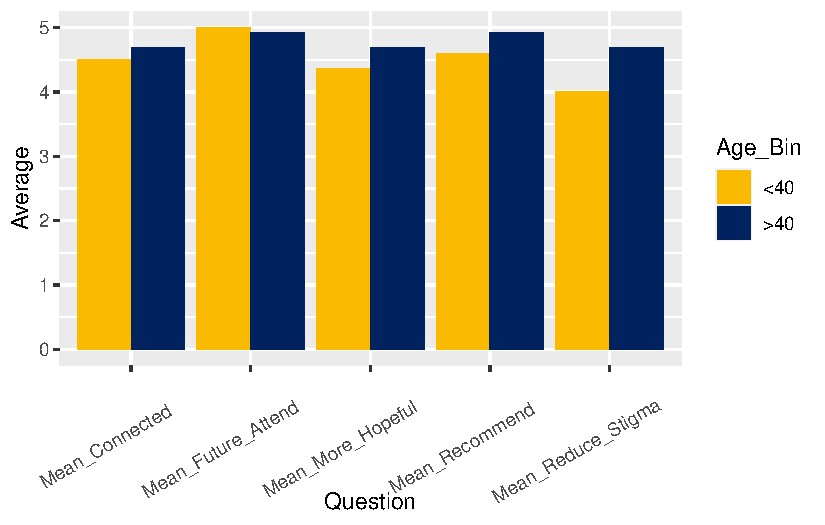
\includegraphics{ytp_post_event_survey_files/figure-pdf/unnamed-chunk-13-1.pdf}

}

\end{figure}

Differences are consistent across the two age brackets. The biggest
difference is observed with the question: \emph{``This event helps
reduce the stigma associated with mental illness.''} responses. The Age
\textless{} 40 bracket hovers around an ``Agree'' for this response. A
\textgreater{} 40 response hovers around 4.5.

\hypertarget{responses-by-event}{%
\subsubsection{Responses by Event}\label{responses-by-event}}

\begin{Shaded}
\begin{Highlighting}[]
\NormalTok{df\_pe\_survey\_clean }\SpecialCharTok{|\textgreater{}} 
  \FunctionTok{filter}\NormalTok{(Event }\SpecialCharTok{==} \StringTok{\textquotesingle{}Fall Hope Garden Planting\textquotesingle{}} \SpecialCharTok{|}
\NormalTok{         Event }\SpecialCharTok{==} \StringTok{\textquotesingle{}Spring Hope Day Event\textquotesingle{}}\NormalTok{) }\SpecialCharTok{|\textgreater{}} 
  \FunctionTok{group\_by}\NormalTok{(Event) }\SpecialCharTok{|\textgreater{}} 
  \FunctionTok{summarise}\NormalTok{(}\AttributeTok{sample\_size =} \FunctionTok{n}\NormalTok{(),}
            \AttributeTok{Mean\_Connected =} \FunctionTok{mean}\NormalTok{(Connected, }\AttributeTok{na.rm=}\NormalTok{T),}
            \AttributeTok{Mean\_Reduce\_Stigma =} \FunctionTok{mean}\NormalTok{(Reduce\_Stigma, }\AttributeTok{na.rm=}\NormalTok{T),}
            \AttributeTok{Mean\_More\_Hopeful =} \FunctionTok{mean}\NormalTok{(More\_Hopeful, }\AttributeTok{na.rm=}\NormalTok{T),}
            \AttributeTok{Mean\_Future\_Attend =} \FunctionTok{mean}\NormalTok{(Future\_Attend, }\AttributeTok{na.rm=}\NormalTok{T),}
            \AttributeTok{Mean\_Recommend =} \FunctionTok{mean}\NormalTok{(Recommend, }\AttributeTok{na.rm=}\NormalTok{T)) }\SpecialCharTok{|\textgreater{}} 
  \FunctionTok{pivot\_longer}\NormalTok{(}\AttributeTok{cols =} \FunctionTok{c}\NormalTok{(}\SpecialCharTok{{-}}\NormalTok{Event, }\SpecialCharTok{{-}}\NormalTok{sample\_size),}
               \AttributeTok{names\_to =} \StringTok{\textquotesingle{}Question\textquotesingle{}}\NormalTok{,}
               \AttributeTok{values\_to =} \StringTok{"Average"}\NormalTok{) }\SpecialCharTok{|\textgreater{}} 
  \FunctionTok{ggplot}\NormalTok{(}\FunctionTok{aes}\NormalTok{(}\AttributeTok{fill =}\NormalTok{ Event, }\AttributeTok{y =}\NormalTok{ Average, }\AttributeTok{x =}\NormalTok{ Question)) }\SpecialCharTok{+}
  \FunctionTok{geom\_bar}\NormalTok{(}\AttributeTok{position=}\StringTok{\textquotesingle{}dodge\textquotesingle{}}\NormalTok{, }\AttributeTok{stat =} \StringTok{\textquotesingle{}identity\textquotesingle{}}\NormalTok{) }\SpecialCharTok{+}
  \FunctionTok{theme}\NormalTok{(}\AttributeTok{axis.text.x =} \FunctionTok{element\_text}\NormalTok{(}\AttributeTok{angle =} \DecValTok{30}\NormalTok{, }\AttributeTok{vjust =} \FloatTok{0.5}\NormalTok{, }\AttributeTok{hjust=}\FloatTok{0.7}\NormalTok{)) }\SpecialCharTok{+}
  \FunctionTok{scale\_fill\_manual}\NormalTok{(}\AttributeTok{values =} \FunctionTok{c}\NormalTok{(}\StringTok{"\#f9ba00"}\NormalTok{,}
                               \StringTok{"\#00235f"}\NormalTok{))}
\end{Highlighting}
\end{Shaded}

\begin{figure}[H]

{\centering 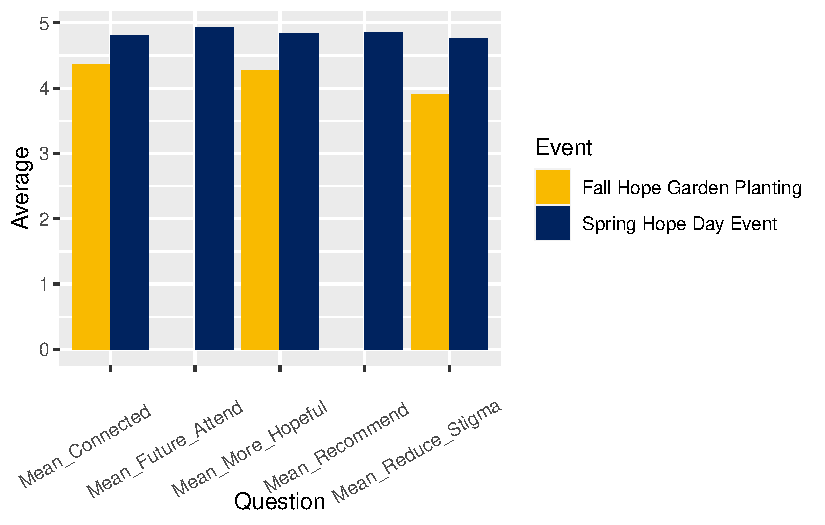
\includegraphics{ytp_post_event_survey_files/figure-pdf/unnamed-chunk-14-1.pdf}

}

\end{figure}

\hypertarget{responses-by-top-two-zipcodes}{%
\subsubsection{Responses by Top Two
Zipcodes}\label{responses-by-top-two-zipcodes}}

Results are mostly consistent between the top two zipcodes: \emph{02360}
and \emph{06830}.

\begin{Shaded}
\begin{Highlighting}[]
\NormalTok{df\_pe\_survey\_clean }\SpecialCharTok{|\textgreater{}} 
  \FunctionTok{filter}\NormalTok{(Zipcode }\SpecialCharTok{==} \StringTok{\textquotesingle{}02360\textquotesingle{}} \SpecialCharTok{|}
\NormalTok{         Zipcode }\SpecialCharTok{==} \StringTok{\textquotesingle{}06830\textquotesingle{}}\NormalTok{) }\SpecialCharTok{|\textgreater{}} 
  \FunctionTok{group\_by}\NormalTok{(Zipcode) }\SpecialCharTok{|\textgreater{}} 
  \FunctionTok{summarise}\NormalTok{(}\AttributeTok{sample\_size =} \FunctionTok{n}\NormalTok{(),}
            \AttributeTok{Mean\_Connected =} \FunctionTok{mean}\NormalTok{(Connected, }\AttributeTok{na.rm=}\NormalTok{T),}
            \AttributeTok{Mean\_Reduce\_Stigma =} \FunctionTok{mean}\NormalTok{(Reduce\_Stigma, }\AttributeTok{na.rm=}\NormalTok{T),}
            \AttributeTok{Mean\_More\_Hopeful =} \FunctionTok{mean}\NormalTok{(More\_Hopeful, }\AttributeTok{na.rm=}\NormalTok{T),}
            \AttributeTok{Mean\_Future\_Attend =} \FunctionTok{mean}\NormalTok{(Future\_Attend, }\AttributeTok{na.rm=}\NormalTok{T),}
            \AttributeTok{Mean\_Recommend =} \FunctionTok{mean}\NormalTok{(Recommend, }\AttributeTok{na.rm=}\NormalTok{T)) }\SpecialCharTok{|\textgreater{}} 
  \FunctionTok{pivot\_longer}\NormalTok{(}\AttributeTok{cols =} \FunctionTok{c}\NormalTok{(}\SpecialCharTok{{-}}\NormalTok{Zipcode, }\SpecialCharTok{{-}}\NormalTok{sample\_size),}
               \AttributeTok{names\_to =} \StringTok{\textquotesingle{}Question\textquotesingle{}}\NormalTok{,}
               \AttributeTok{values\_to =} \StringTok{"Average"}\NormalTok{) }\SpecialCharTok{|\textgreater{}} 
  \FunctionTok{ggplot}\NormalTok{(}\FunctionTok{aes}\NormalTok{(}\AttributeTok{fill =}\NormalTok{ Zipcode, }\AttributeTok{y =}\NormalTok{ Average, }\AttributeTok{x =}\NormalTok{ Question)) }\SpecialCharTok{+}
  \FunctionTok{geom\_bar}\NormalTok{(}\AttributeTok{position=}\StringTok{\textquotesingle{}dodge\textquotesingle{}}\NormalTok{, }\AttributeTok{stat =} \StringTok{\textquotesingle{}identity\textquotesingle{}}\NormalTok{) }\SpecialCharTok{+}
  \FunctionTok{theme}\NormalTok{(}\AttributeTok{axis.text.x =} \FunctionTok{element\_text}\NormalTok{(}\AttributeTok{angle =} \DecValTok{30}\NormalTok{, }\AttributeTok{vjust =} \FloatTok{0.5}\NormalTok{, }\AttributeTok{hjust=}\FloatTok{0.7}\NormalTok{)) }\SpecialCharTok{+}
  \FunctionTok{scale\_fill\_manual}\NormalTok{(}\AttributeTok{values =} \FunctionTok{c}\NormalTok{(}\StringTok{"\#f9ba00"}\NormalTok{,}
                               \StringTok{"\#00235f"}\NormalTok{))}
\end{Highlighting}
\end{Shaded}

\begin{figure}[H]

{\centering 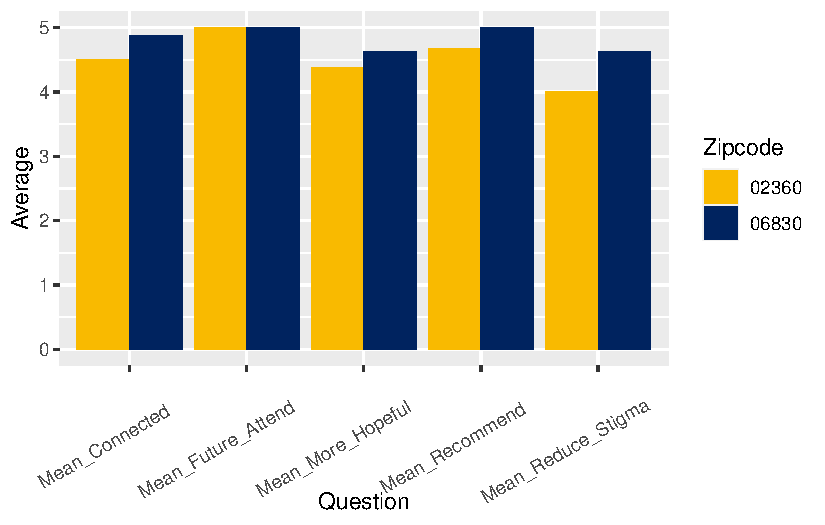
\includegraphics{ytp_post_event_survey_files/figure-pdf/unnamed-chunk-15-1.pdf}

}

\end{figure}

\hypertarget{responses-by-gender}{%
\subsection{Responses by Gender}\label{responses-by-gender}}

\begin{Shaded}
\begin{Highlighting}[]
\NormalTok{df\_pe\_survey\_clean }\SpecialCharTok{|\textgreater{}} 
  \FunctionTok{group\_by}\NormalTok{(Gender) }\SpecialCharTok{|\textgreater{}} 
  \FunctionTok{summarise}\NormalTok{(}\AttributeTok{sample\_size =} \FunctionTok{n}\NormalTok{(),}
            \AttributeTok{Mean\_Connected =} \FunctionTok{mean}\NormalTok{(Connected, }\AttributeTok{na.rm=}\NormalTok{T),}
            \AttributeTok{Mean\_Reduce\_Stigma =} \FunctionTok{mean}\NormalTok{(Reduce\_Stigma, }\AttributeTok{na.rm=}\NormalTok{T),}
            \AttributeTok{Mean\_More\_Hopeful =} \FunctionTok{mean}\NormalTok{(More\_Hopeful, }\AttributeTok{na.rm=}\NormalTok{T),}
            \AttributeTok{Mean\_Future\_Attend =} \FunctionTok{mean}\NormalTok{(Future\_Attend, }\AttributeTok{na.rm=}\NormalTok{T),}
            \AttributeTok{Mean\_Recommend =} \FunctionTok{mean}\NormalTok{(Recommend, }\AttributeTok{na.rm=}\NormalTok{T)) }\SpecialCharTok{|\textgreater{}} 
  \FunctionTok{pivot\_longer}\NormalTok{(}\AttributeTok{cols =} \FunctionTok{c}\NormalTok{(}\SpecialCharTok{{-}}\NormalTok{Gender, }\SpecialCharTok{{-}}\NormalTok{sample\_size),}
               \AttributeTok{names\_to =} \StringTok{\textquotesingle{}Question\textquotesingle{}}\NormalTok{,}
               \AttributeTok{values\_to =} \StringTok{"Average"}\NormalTok{) }\SpecialCharTok{|\textgreater{}} 
  \FunctionTok{ggplot}\NormalTok{(}\FunctionTok{aes}\NormalTok{(}\AttributeTok{fill =}\NormalTok{ Gender, }\AttributeTok{y =}\NormalTok{ Average, }\AttributeTok{x =}\NormalTok{ Question)) }\SpecialCharTok{+}
  \FunctionTok{geom\_bar}\NormalTok{(}\AttributeTok{position=}\StringTok{\textquotesingle{}dodge\textquotesingle{}}\NormalTok{, }\AttributeTok{stat =} \StringTok{\textquotesingle{}identity\textquotesingle{}}\NormalTok{) }\SpecialCharTok{+}
  \FunctionTok{theme}\NormalTok{(}\AttributeTok{axis.text.x =} \FunctionTok{element\_text}\NormalTok{(}\AttributeTok{angle =} \DecValTok{30}\NormalTok{, }\AttributeTok{vjust =} \FloatTok{0.5}\NormalTok{, }\AttributeTok{hjust=}\FloatTok{0.7}\NormalTok{)) }\SpecialCharTok{+}
  \FunctionTok{scale\_fill\_manual}\NormalTok{(}\AttributeTok{values =} \FunctionTok{c}\NormalTok{(}\StringTok{"\#f9ba00"}\NormalTok{,}
                               \StringTok{"\#00235f"}\NormalTok{))}
\end{Highlighting}
\end{Shaded}

\begin{figure}[H]

{\centering 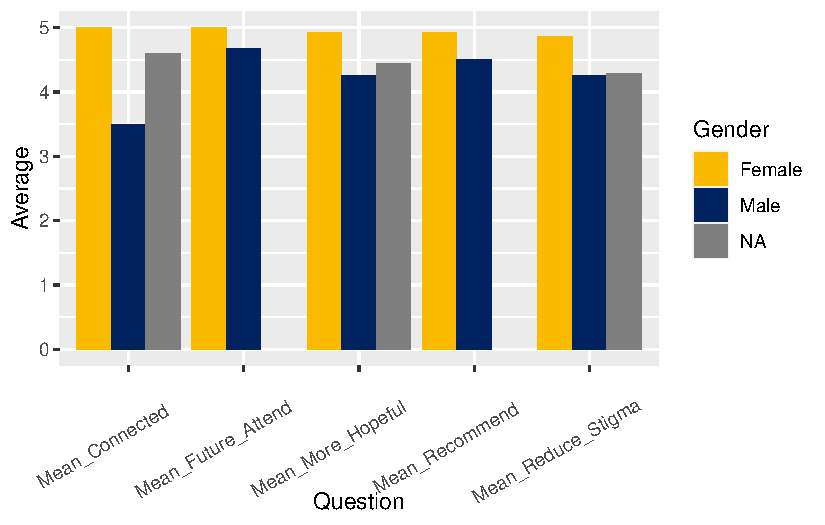
\includegraphics{ytp_post_event_survey_files/figure-pdf/unnamed-chunk-16-1.pdf}

}

\end{figure}

\hypertarget{responses-by-age-bin-1}{%
\subsubsection{Responses by Age Bin}\label{responses-by-age-bin-1}}

\begin{Shaded}
\begin{Highlighting}[]
\NormalTok{df\_pe\_survey\_clean }\SpecialCharTok{|\textgreater{}} 
  \FunctionTok{filter}\NormalTok{(Join\_Network }\SpecialCharTok{==} \StringTok{\textquotesingle{}Student\textquotesingle{}} \SpecialCharTok{|}
\NormalTok{           Join\_Network }\SpecialCharTok{==} \StringTok{\textquotesingle{}Community Member\textquotesingle{}} \SpecialCharTok{|}
\NormalTok{           Join\_Network }\SpecialCharTok{==} \StringTok{\textquotesingle{}Educator\textquotesingle{}}\NormalTok{) }\SpecialCharTok{|\textgreater{}} 
  \FunctionTok{group\_by}\NormalTok{(Join\_Network) }\SpecialCharTok{|\textgreater{}} 
  \FunctionTok{summarise}\NormalTok{(}\AttributeTok{sample\_size =} \FunctionTok{n}\NormalTok{(),}
            \AttributeTok{Mean\_Connected =} \FunctionTok{mean}\NormalTok{(Connected, }\AttributeTok{na.rm=}\NormalTok{T),}
            \AttributeTok{Mean\_Reduce\_Stigma =} \FunctionTok{mean}\NormalTok{(Reduce\_Stigma, }\AttributeTok{na.rm=}\NormalTok{T),}
            \AttributeTok{Mean\_More\_Hopeful =} \FunctionTok{mean}\NormalTok{(More\_Hopeful, }\AttributeTok{na.rm=}\NormalTok{T),}
            \AttributeTok{Mean\_Future\_Attend =} \FunctionTok{mean}\NormalTok{(Future\_Attend, }\AttributeTok{na.rm=}\NormalTok{T),}
            \AttributeTok{Mean\_Recommend =} \FunctionTok{mean}\NormalTok{(Recommend, }\AttributeTok{na.rm=}\NormalTok{T)) }\SpecialCharTok{|\textgreater{}} 
  \FunctionTok{pivot\_longer}\NormalTok{(}\AttributeTok{cols =} \FunctionTok{c}\NormalTok{(}\SpecialCharTok{{-}}\NormalTok{Join\_Network, }\SpecialCharTok{{-}}\NormalTok{sample\_size),}
               \AttributeTok{names\_to =} \StringTok{\textquotesingle{}Question\textquotesingle{}}\NormalTok{,}
               \AttributeTok{values\_to =} \StringTok{"Average"}\NormalTok{) }\SpecialCharTok{|\textgreater{}} 
  \FunctionTok{ggplot}\NormalTok{(}\FunctionTok{aes}\NormalTok{(}\AttributeTok{fill =}\NormalTok{ Join\_Network, }\AttributeTok{y =}\NormalTok{ Average, }\AttributeTok{x =}\NormalTok{ Question)) }\SpecialCharTok{+}
  \FunctionTok{geom\_bar}\NormalTok{(}\AttributeTok{position=}\StringTok{\textquotesingle{}dodge\textquotesingle{}}\NormalTok{, }\AttributeTok{stat =} \StringTok{\textquotesingle{}identity\textquotesingle{}}\NormalTok{) }\SpecialCharTok{+}
  \FunctionTok{theme}\NormalTok{(}\AttributeTok{axis.text.x =} \FunctionTok{element\_text}\NormalTok{(}\AttributeTok{angle =} \DecValTok{30}\NormalTok{, }\AttributeTok{vjust =} \FloatTok{0.5}\NormalTok{, }\AttributeTok{hjust=}\FloatTok{0.7}\NormalTok{)) }\SpecialCharTok{+}
  \FunctionTok{scale\_fill\_manual}\NormalTok{(}\AttributeTok{values =} \FunctionTok{c}\NormalTok{(}\StringTok{"\#f9ba00"}\NormalTok{,}
                               \StringTok{"\#00235f"}\NormalTok{,}
                               \StringTok{\textquotesingle{}darkgray\textquotesingle{}}\NormalTok{))}
\end{Highlighting}
\end{Shaded}

\begin{figure}[H]

{\centering 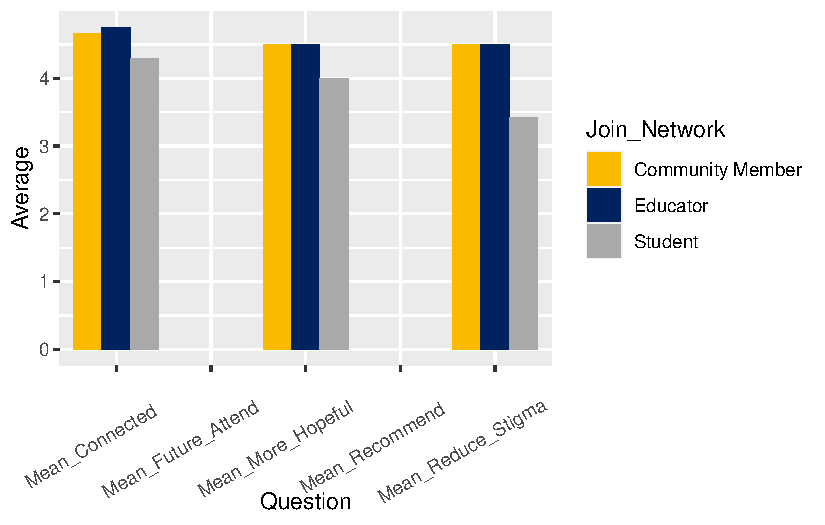
\includegraphics{ytp_post_event_survey_files/figure-pdf/unnamed-chunk-17-1.pdf}

}

\end{figure}

Most responses across the three types of members is in-line with one
another. Though for students, the ability to reduce stigma with these
events is lower than Educators and Community Members. This could be an
area for further research.

\hypertarget{correlation-analysis}{%
\subsection{Correlation Analysis}\label{correlation-analysis}}

A correlation is a trend between two different numbers. The scale of a
correlation is -1 through +1. A -1 correlation would indicate a perfect
inverse relationship, as one goes up, the other goes down. A positive
correlation would indicate as one variable increases, so does the other
variable. For example, temperature and number of sunburns. If the
correlation is +1, this would indicate that as temperature increases, so
does the number of sunburns, which makes perfect sense. A negative
correlation with this example could be with snowfall. As temperatures
increase, snowfall decreases. This is a negative correlation.

In our survey context, we intend to take a look at how our various scale
questions correlate with one another. We'd like to see mostly positive
correlations, where the more somebody felt connected to an event, the
higher probability that they will tell their friends and family about
it.

\begin{Shaded}
\begin{Highlighting}[]
\NormalTok{df\_corr }\OtherTok{\textless{}{-}}
\NormalTok{  df\_pe\_survey\_clean }\SpecialCharTok{\%\textgreater{}\%}
  \FunctionTok{select}\NormalTok{(Connected,}
\NormalTok{         Reduce\_Stigma,}
\NormalTok{         More\_Hopeful,}
\NormalTok{         Future\_Attend,}
\NormalTok{         Recommend)}

\NormalTok{M\_corr }\OtherTok{=} \FunctionTok{cor}\NormalTok{(df\_corr, }\AttributeTok{use =} \StringTok{"pairwise.complete.obs"}\NormalTok{)}
\NormalTok{M\_test }\OtherTok{=} \FunctionTok{cor.mtest}\NormalTok{(df\_corr, }\AttributeTok{conf.level =}\NormalTok{ .}\DecValTok{95}\NormalTok{)}

\FunctionTok{corrplot}\NormalTok{(}
\NormalTok{  M\_corr,}
  \AttributeTok{method =} \StringTok{\textquotesingle{}number\textquotesingle{}}\NormalTok{,}
  \AttributeTok{diag =} \ConstantTok{FALSE}\NormalTok{,}
  \AttributeTok{type =} \StringTok{\textquotesingle{}upper\textquotesingle{}}\NormalTok{,}
  \AttributeTok{col =} \FunctionTok{COL2}\NormalTok{(}\StringTok{\textquotesingle{}RdBu\textquotesingle{}}\NormalTok{, }\DecValTok{2}\NormalTok{),}
  \AttributeTok{p.mat =}\NormalTok{ M\_test}\SpecialCharTok{$}\NormalTok{p,}
  \AttributeTok{sig.level =}\NormalTok{ .}\DecValTok{05}\NormalTok{,}
  \AttributeTok{pch.cex =} \DecValTok{2}\NormalTok{,}
  \AttributeTok{pch.col =} \StringTok{"darkgray"}\NormalTok{,}
  \AttributeTok{tl.col =} \StringTok{"black"}\NormalTok{,}
  \AttributeTok{tl.srt =} \DecValTok{45}\NormalTok{,}
  \CommentTok{\#Text label color and rotation}
  \AttributeTok{tl.cex =} \DecValTok{1} \SpecialCharTok{/} \FunctionTok{par}\NormalTok{(}\StringTok{"cex"}\NormalTok{),}
  \AttributeTok{cl.cex =} \DecValTok{1} \SpecialCharTok{/} \FunctionTok{par}\NormalTok{(}\StringTok{"cex"}\NormalTok{)}
\NormalTok{)}
\end{Highlighting}
\end{Shaded}

\begin{figure}[H]

{\centering 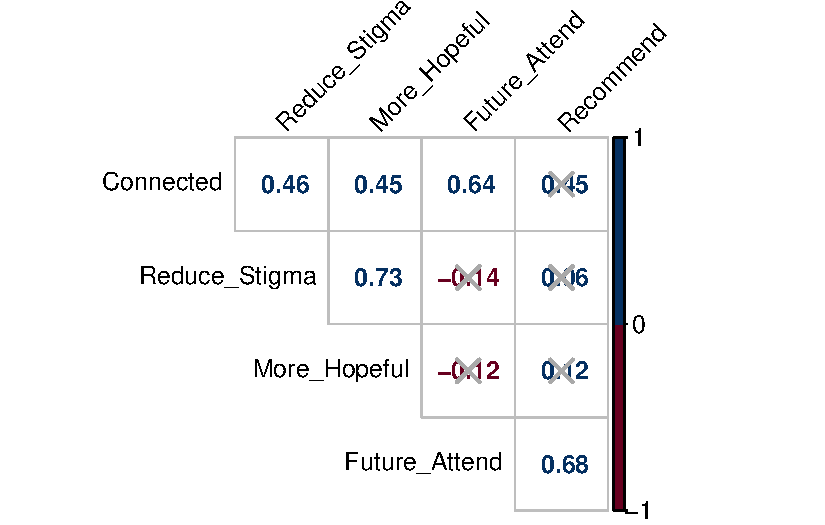
\includegraphics{ytp_post_event_survey_files/figure-pdf/unnamed-chunk-18-1.pdf}

}

\end{figure}

We have a lot of statistically significant findings from the survey
questions. Some takeaways include:

\begin{enumerate}
\def\labelenumi{\arabic{enumi}.}
\tightlist
\item
  People who are more likely to attend a future event are also more
  likely to recommend the event to a friend or family member.
\item
  People who believe the event is reducing stigma are also more likely
  to feel hopeful.
\item
  People who came to the event and feel more connected are also more
  likely to attend the event in the future.
\item
  An interesting observation is that people who are less hopeful also
  are more likely to attend a future event (-0.12 correlation, not
  statistically significant). This is an interesting finding because it
  shows that there are people who are willing to put in the work to
  continually come to events to become more optimistic/hopeful.
\end{enumerate}

\hypertarget{time-series-analysis-of-reducing-stigma}{%
\subsection{Time Series Analysis of Reducing
Stigma}\label{time-series-analysis-of-reducing-stigma}}

We take a look at the trend of responses over time:

\begin{Shaded}
\begin{Highlighting}[]
\NormalTok{df\_pe\_survey\_clean }\SpecialCharTok{|\textgreater{}}
  \FunctionTok{mutate}\NormalTok{(}\AttributeTok{Date =} \FunctionTok{as.Date}\NormalTok{(Date, }\AttributeTok{format =} \StringTok{"\%m/\%d/\%Y"}\NormalTok{)) }\SpecialCharTok{|\textgreater{}}
  \FunctionTok{group\_by}\NormalTok{(Date) }\SpecialCharTok{|\textgreater{}}
  \FunctionTok{summarise}\NormalTok{(}\AttributeTok{Mean\_Stigma =} \FunctionTok{mean}\NormalTok{(Reduce\_Stigma, }\AttributeTok{na.rm =} \ConstantTok{TRUE}\NormalTok{)) }\SpecialCharTok{|\textgreater{}}
  \FunctionTok{ggplot}\NormalTok{(}\FunctionTok{aes}\NormalTok{(}\AttributeTok{x =}\NormalTok{ Date, }\AttributeTok{y =}\NormalTok{ Mean\_Stigma)) }\SpecialCharTok{+}
  \FunctionTok{geom\_line}\NormalTok{(}\AttributeTok{color =} \StringTok{"steelblue"}\NormalTok{) }\SpecialCharTok{+}
  \FunctionTok{geom\_point}\NormalTok{() }\SpecialCharTok{+}
  \FunctionTok{geom\_smooth}\NormalTok{() }\SpecialCharTok{+}
  \FunctionTok{xlab}\NormalTok{(}\StringTok{""}\NormalTok{) }\SpecialCharTok{+}
  \FunctionTok{theme\_bw}\NormalTok{() }\SpecialCharTok{+}
  \FunctionTok{theme}\NormalTok{(}\AttributeTok{axis.text.x =} \FunctionTok{element\_text}\NormalTok{(}\AttributeTok{angle =} \DecValTok{60}\NormalTok{, }\AttributeTok{hjust =} \DecValTok{1}\NormalTok{))}\CommentTok{\# +}
\end{Highlighting}
\end{Shaded}

\begin{figure}[H]

{\centering 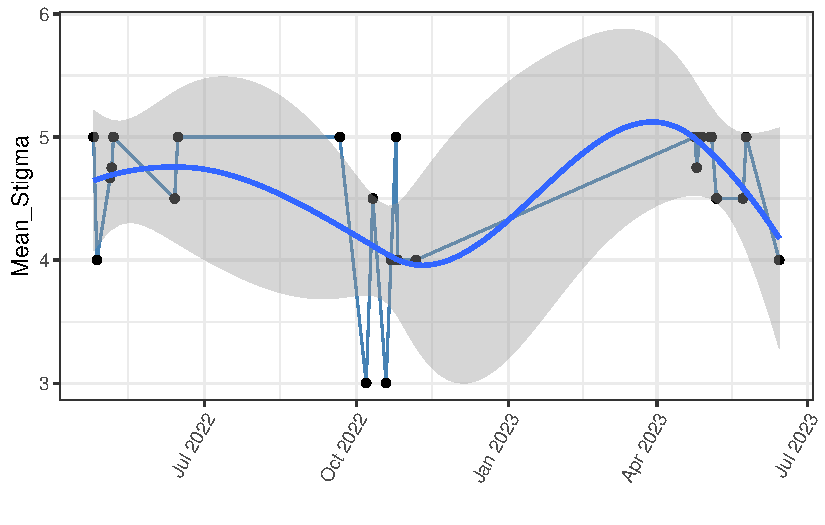
\includegraphics{ytp_post_event_survey_files/figure-pdf/unnamed-chunk-19-1.pdf}

}

\end{figure}

\begin{Shaded}
\begin{Highlighting}[]
  \CommentTok{\#scale\_x\_date(limit = c(as.Date("2017{-}01{-}01"), as.Date("2017{-}02{-}11"))) +}
  \CommentTok{\#ylim(0, 1.5)}
\end{Highlighting}
\end{Shaded}

Here we are attempting to model average Stigma ratings over time. The
hope would be that over time, these series of events help reduce the
stigma associated with mental illness.

\hypertarget{time-series-analysis-of-recommend-to-a-friend}{%
\subsection{Time Series Analysis of Recommend to a
Friend}\label{time-series-analysis-of-recommend-to-a-friend}}

\begin{Shaded}
\begin{Highlighting}[]
\NormalTok{df\_pe\_survey\_clean }\SpecialCharTok{|\textgreater{}}
  \FunctionTok{mutate}\NormalTok{(}\AttributeTok{Date =} \FunctionTok{as.Date}\NormalTok{(Date, }\AttributeTok{format =} \StringTok{"\%m/\%d/\%Y"}\NormalTok{)) }\SpecialCharTok{|\textgreater{}}
  \FunctionTok{group\_by}\NormalTok{(Date) }\SpecialCharTok{|\textgreater{}}
  \FunctionTok{summarise}\NormalTok{(}\AttributeTok{Mean\_Recommend =} \FunctionTok{mean}\NormalTok{(Recommend, }\AttributeTok{na.rm =} \ConstantTok{TRUE}\NormalTok{)) }\SpecialCharTok{|\textgreater{}}
  \FunctionTok{filter}\NormalTok{(}\SpecialCharTok{!}\FunctionTok{is.na}\NormalTok{(Mean\_Recommend)) }\SpecialCharTok{|\textgreater{}} 
  \FunctionTok{ggplot}\NormalTok{(}\FunctionTok{aes}\NormalTok{(}\AttributeTok{x =}\NormalTok{ Date, }\AttributeTok{y =}\NormalTok{ Mean\_Recommend)) }\SpecialCharTok{+}
  \FunctionTok{geom\_line}\NormalTok{(}\AttributeTok{color =} \StringTok{"steelblue"}\NormalTok{) }\SpecialCharTok{+}
  \FunctionTok{geom\_point}\NormalTok{() }\SpecialCharTok{+}
  \FunctionTok{geom\_smooth}\NormalTok{() }\SpecialCharTok{+}
  \FunctionTok{xlab}\NormalTok{(}\StringTok{""}\NormalTok{) }\SpecialCharTok{+}
  \FunctionTok{theme\_bw}\NormalTok{() }\SpecialCharTok{+}
  \FunctionTok{theme}\NormalTok{(}\AttributeTok{axis.text.x =} \FunctionTok{element\_text}\NormalTok{(}\AttributeTok{angle =} \DecValTok{60}\NormalTok{, }\AttributeTok{hjust =} \DecValTok{1}\NormalTok{))}\CommentTok{\# +}
\end{Highlighting}
\end{Shaded}

\begin{figure}[H]

{\centering 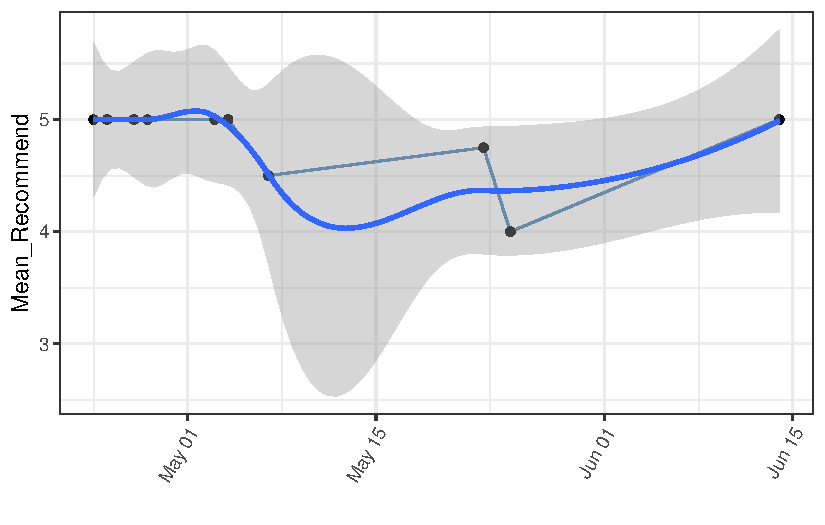
\includegraphics{ytp_post_event_survey_files/figure-pdf/unnamed-chunk-20-1.pdf}

}

\end{figure}

\begin{Shaded}
\begin{Highlighting}[]
  \CommentTok{\#scale\_x\_date(limit = c(as.Date("2017{-}01{-}01"), as.Date("2017{-}02{-}11"))) +}
  \CommentTok{\#ylim(0, 1.5)}
\end{Highlighting}
\end{Shaded}

This question is a bit too recent for us to be able to analyze
effectively

\hypertarget{time-series-of-future-attendance}{%
\subsection{Time Series of Future
Attendance}\label{time-series-of-future-attendance}}

\begin{Shaded}
\begin{Highlighting}[]
\NormalTok{df\_pe\_survey\_clean }\SpecialCharTok{|\textgreater{}}
  \FunctionTok{mutate}\NormalTok{(}\AttributeTok{Date =} \FunctionTok{as.Date}\NormalTok{(Date, }\AttributeTok{format =} \StringTok{"\%m/\%d/\%Y"}\NormalTok{)) }\SpecialCharTok{|\textgreater{}}
  \FunctionTok{group\_by}\NormalTok{(Date) }\SpecialCharTok{|\textgreater{}}
  \FunctionTok{summarise}\NormalTok{(}\AttributeTok{Mean\_Attend =} \FunctionTok{mean}\NormalTok{(Future\_Attend, }\AttributeTok{na.rm =} \ConstantTok{TRUE}\NormalTok{)) }\SpecialCharTok{|\textgreater{}}
  \FunctionTok{filter}\NormalTok{(}\SpecialCharTok{!}\FunctionTok{is.na}\NormalTok{(Mean\_Attend)) }\SpecialCharTok{|\textgreater{}} 
  \FunctionTok{ggplot}\NormalTok{(}\FunctionTok{aes}\NormalTok{(}\AttributeTok{x =}\NormalTok{ Date, }\AttributeTok{y =}\NormalTok{ Mean\_Attend)) }\SpecialCharTok{+}
  \FunctionTok{geom\_line}\NormalTok{(}\AttributeTok{color =} \StringTok{"steelblue"}\NormalTok{) }\SpecialCharTok{+}
  \FunctionTok{geom\_point}\NormalTok{() }\SpecialCharTok{+}
  \FunctionTok{geom\_smooth}\NormalTok{() }\SpecialCharTok{+}
  \FunctionTok{xlab}\NormalTok{(}\StringTok{""}\NormalTok{) }\SpecialCharTok{+}
  \FunctionTok{theme\_bw}\NormalTok{() }\SpecialCharTok{+}
  \FunctionTok{theme}\NormalTok{(}\AttributeTok{axis.text.x =} \FunctionTok{element\_text}\NormalTok{(}\AttributeTok{angle =} \DecValTok{60}\NormalTok{, }\AttributeTok{hjust =} \DecValTok{1}\NormalTok{))}\CommentTok{\# +}
\end{Highlighting}
\end{Shaded}

\begin{figure}[H]

{\centering 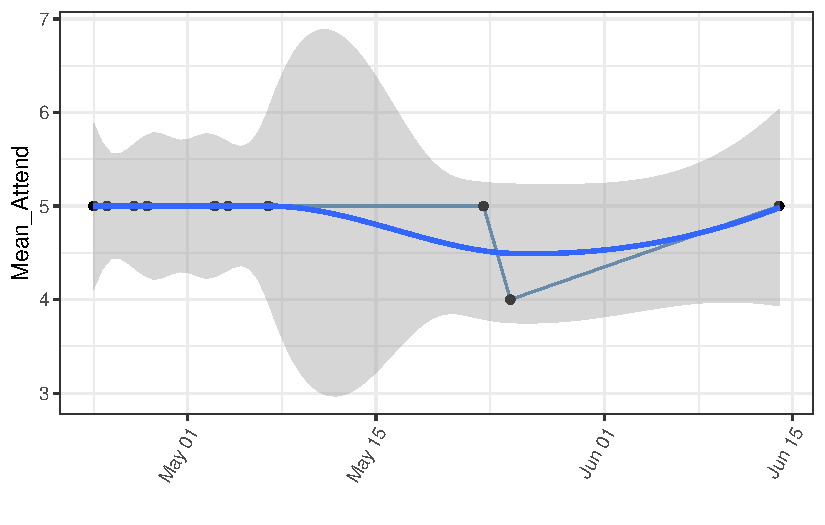
\includegraphics{ytp_post_event_survey_files/figure-pdf/unnamed-chunk-21-1.pdf}

}

\end{figure}

\begin{Shaded}
\begin{Highlighting}[]
  \CommentTok{\#scale\_x\_date(limit = c(as.Date("2017{-}01{-}01"), as.Date("2017{-}02{-}11"))) +}
  \CommentTok{\#ylim(0, 1.5)}
\end{Highlighting}
\end{Shaded}

\hypertarget{text-analysis-how-can-we-improve}{%
\subsection{Text Analysis: ``How can we
improve?''}\label{text-analysis-how-can-we-improve}}

This question was difficult to decipher because it seems to be a
catch-all for any open-ended text that people want to express about
these events in general. Most of the comments in this field were not
recommendations at all, but rather, praise about the event. For example:

\begin{itemize}
\item
  It was a lot of fun, and I loved it!
\item
  I was thrilled with the participation in the hooray walk. It was
  amazing to have activities for participants at the end.
\item
  It was fantastic!
\end{itemize}

These types of comments were mixed in with actual recommendations, such
as:

\begin{itemize}
\item
  More widespread event promotion and publicity.
\item
  I feel that we tried to put 2 events in one. I think the panel
  discussion should have been the following night.
\end{itemize}

Therefore, any sort of word cloud analysis that we'd like to implement
will be mixed in terms of how the words should be interpreted. As a
majority of the comments were positive feedback, we can interpret the
word cloud as representing general feedback about the performance of YTP
over the last year.

\begin{Shaded}
\begin{Highlighting}[]
\NormalTok{tokens\_clean }\OtherTok{\textless{}{-}}
\NormalTok{df\_pe\_survey\_clean }\SpecialCharTok{|\textgreater{}} 
  \FunctionTok{unnest\_tokens}\NormalTok{(}\AttributeTok{input =}\NormalTok{ Text\_Improve,}\AttributeTok{output =} \StringTok{\textquotesingle{}word\textquotesingle{}}\NormalTok{) }\SpecialCharTok{|\textgreater{}} 
  \FunctionTok{select}\NormalTok{(word) }\SpecialCharTok{|\textgreater{}} 
  \FunctionTok{anti\_join}\NormalTok{(stop\_words) }\SpecialCharTok{|\textgreater{}} 
  \FunctionTok{filter}\NormalTok{(}\SpecialCharTok{!}\FunctionTok{is.na}\NormalTok{(word)) }\SpecialCharTok{|\textgreater{}} 
  \FunctionTok{count}\NormalTok{(word)}

\NormalTok{pal }\OtherTok{\textless{}{-}} \FunctionTok{brewer.pal}\NormalTok{(}\DecValTok{8}\NormalTok{,}\StringTok{"Dark2"}\NormalTok{)}

\NormalTok{tokens\_clean }\SpecialCharTok{\%\textgreater{}\%} 
  \FunctionTok{with}\NormalTok{(}\FunctionTok{wordcloud}\NormalTok{(word, n, }\AttributeTok{random.order =} \ConstantTok{FALSE}\NormalTok{, }\AttributeTok{max.words =} \DecValTok{25}\NormalTok{, }\AttributeTok{colors=}\NormalTok{pal))}
\end{Highlighting}
\end{Shaded}

\begin{figure}[H]

{\centering 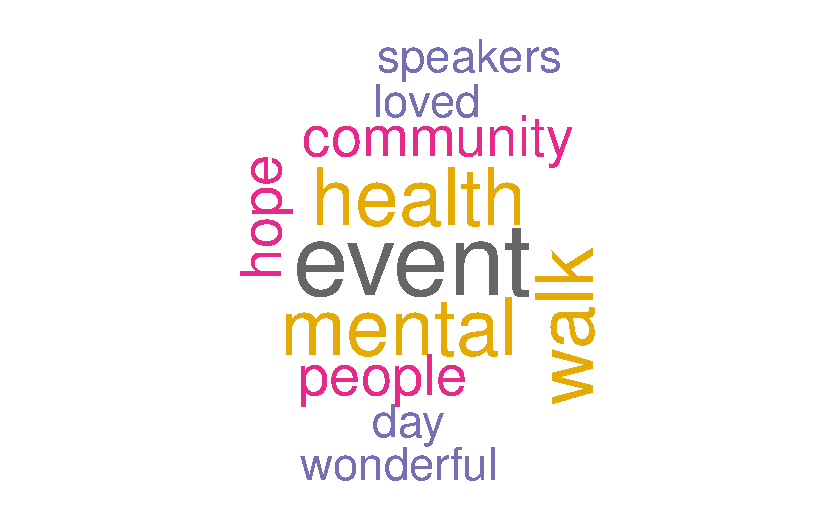
\includegraphics{ytp_post_event_survey_files/figure-pdf/unnamed-chunk-22-1.pdf}

}

\end{figure}



\end{document}
